%%%%%%%%%%%%%%%%%%%%%%%%%%%%%%%%%%%%%%%%%%%%%%%%%%%%%%%%%%%%%%%%%%
%%%%%%%%			BACKGROUND
%%%%%%%%%%%%%%%%%%%%%%%%%%%%%%%%%%%%%%%%%%%%%%%%%%%%%%%%%%%%%%%%%%

\section{Background \& Literature Review}

%%\subsection{Introductory Statement}
%%\paragraph{} 
%%Due to my personal experience working as a trainee electrical engineer for an electrical contractor I have a stronger understanding of power systems in the construction industry than most students at my level. This project will be focusing on a designs and simulations to produce deliverables.  

%%%%%%%%%%%%%%%%%%%%%%%%%%%%%%%%%%%%%%%%%%%%%%%%%%%%%%%%%%%%%%%%%%
%%%%%%%%			LITERATURE REVIEW
%%%%%%%%%%%%%%%%%%%%%%%%%%%%%%%%%%%%%%%%%%%%%%%%%%%%%%%%%%%%%%%%%%

\subsection{Literature Review}

%%%%%%% POWER SYSTEMS %%%%%%%%%%%%%
%%%%%%% POWER SYSTEMS %%%%%%%%%%%%%
%%%%%%% POWER SYSTEMS %%%%%%%%%%%%%
%%%%%%% POWER SYSTEMS %%%%%%%%%%%%%
%%%%%%% POWER SYSTEMS %%%%%%%%%%%%%


\subsubsection{Power Systems}

\paragraph{Existing Power Distribution Systems}
~\\
%New Paragraph
Power systems consist of four major sections; generation, transmission, distribution and loads shown in Figure \ref{fig:ExistingPower}. AC electricity is generated in power plants and sent through high voltage transmission lines to substations and distributed to switchboards for use in residential, commercial and industrial areas \cite{Amin2011}. In order to transport electricity over large distances (excess of 2km) without severe losses, very high voltage and low current is used \cite{Amin2011}. This is voltage is lowered and current increased by a transformer at the substation and again at the residence. For electricity to reach the home and be utilised for devices there must be safety mechanisms installed to ensure damage is not done to the user or devices. The protective devices requiring consideration throughout this project will be fuses, circuit breakers and switchboards \cite{UnitedStatesDepartmentoftheInterior2000}. These devices are placed through the circuit to protect the more expensive equipment closer to the transformer and grid.  

\begin{figure}[H]
	\hfill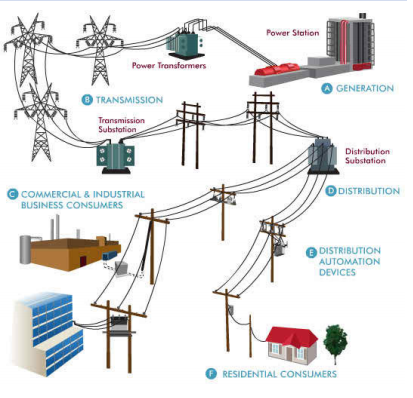
\includegraphics[width = 100mm]{images/Power_Distro}\hspace*{\fill}
	\caption{Existing Common Power Distribution Methods \cite{Active2015}}
	\label{fig:ExistingPower}
\end{figure}

\paragraph{Commercial and Industrial Power Systems}
~\\
%New Paragraph
There are relatively large differences between home and commercial power systems. A home application is fairly simple wih a transformer feeding electricity into one distribution board (DB) or switchboard (SB) that provides safety mechanisms along with circuit breakers for the home circuits. In a commercial setting, the loads are far higher and require a stable connection \cite{Baran2003}. For an apartment complex, shopping centre or business building, the supplies are generally separated into buses in order to identify separate requirements or areas. The requirements could be essential items (including emergency lifts, safety equipment or machines that cannot be stopped) or non-essentials (tenancies or general equipment). Additionally it can be used to separate the entire building's load over towers or zones to minimise faults. Figure \ref{fig:SLD} represents a single line diagram showing the two separate buses for a design. 

\begin{figure}[H]
	\hfill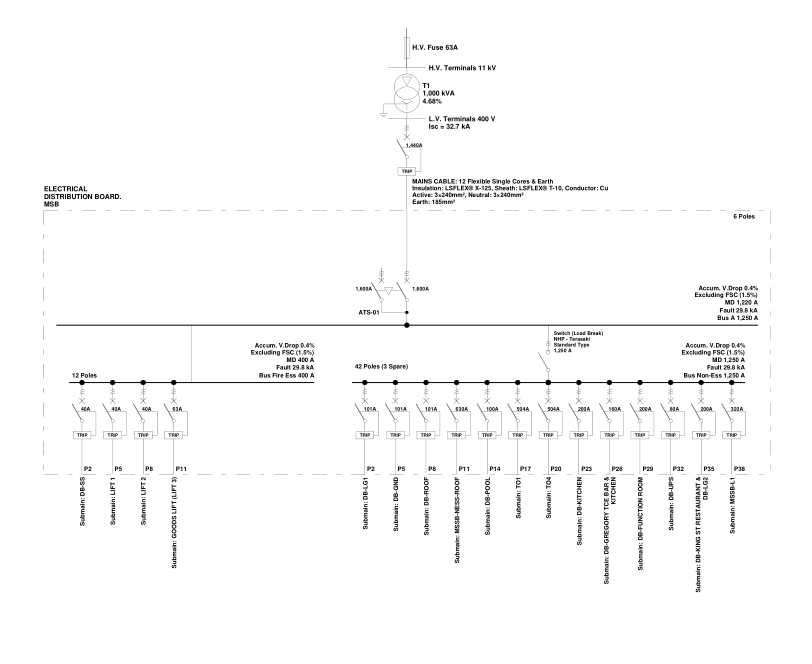
\includegraphics[width = 160mm, height = 110mm]{images/PCad_SLD}\hspace*{\fill}
	\caption{Example of Single Line Diagram - Hotel/Multi-Residential Building}
	\label{fig:SLD}
\end{figure} 

\paragraph{Electrical Safety Mechanisms}
~\\
%New Paragraph
For electricity to each the home and be utilised for devices there must be safety mechanisms installed to ensure damage is not done to the user or devices. The protective devices requiring consideration throughout this project will be fuses, circuit breakers and switchboards \cite{UnitedStatesDepartmentoftheInterior2000}. These devices are placed through the circuit to protect the more expensive equipment closer to the transformer and grid. A fuse is a simple device that acts as a sacrificial lamb for the protection of the more expensive devices. An internal wire will melt when too much current flows through therefore interrupting the connection \cite{UnitedStatesDepartmentoftheInterior2000}. A circuit breaker is a smarter and re-usable version of a fuse that is triggered by over current, overloads or shirt circuits to fulfil the same purpose \cite{UnitedStatesDepartmentoftheInterior2000}. The switchboard is a device that connects a home or building to the electrical grid and allows for individual circuits to be run for different purposes throughout the complex \cite{UnitedStatesDepartmentoftheInterior2000}.

\paragraph{Summary of Power Systems}
~\\
This section covered the main concepts of power distribution systems. This knowledge will be integral to understanding where the extra-low voltage design will begin and how to efficiently incorporate it with existing infrastructure. The safety mechanisms will have to be considered for a system that is not based on traditional AC concepts.  

%%%%%%% REGULATIONS %%%%%%%%%%%%%
%%%%%%% REGULATIONS %%%%%%%%%%%%%
%%%%%%% REGULATIONS %%%%%%%%%%%%%
%%%%%%% REGULATIONS %%%%%%%%%%%%%
%%%%%%% REGULATIONS %%%%%%%%%%%%%
%%%%%%% REGULATIONS %%%%%%%%%%%%%


\subsubsection{Regulations}

\paragraph{Standards}
~\\
%New Paragraph
Australian standards will be an integral part of this project. If the rules and regulations are not adhered to, the devised system will not be legally approved for installation. There are four standards that will be relevant to this report; AS3000, AS3008, AS1680 and AS3015. The AS/NZS 3000 covers the standards related to electrical installations or wiring rules within Australia and New Zealand \cite{StandardsAustralia2007}. These standards will be the main reference point. The AS/NZS 3008 which are the regulations specifically related to electrical installations and cable specifications will be vital \cite{StandardsAustralia2010}. An additional set of standards that will be used for initial calculations and estimation of building load requires is AS/NZS 1680 which are the lighting regulations and requirements for interiors and workplaces \cite{StandardsAustralia2006_2}. These standards outline the lux levels required by rooms depending according to their purpose allowing 3D models to be created. The AS/NZS 3015 specifically dictates the rules with regards to electrical installations of extra-low voltage direct current power supplies and services earthing within public telecommunications \cite{StandardsAustralia2004}.

\paragraph{Voltage Levels as per Australian Standards}
~\\
%New Paragraph
The Australian Standards (AS/NZS 3000: Wiring Rules) outline the specific voltage levels that distinguish circuits \cite{StandardsAustralia2007}. This information is required for both separate standards related to the design and distribution of each chosen voltage level. Extra-Low Voltage is any voltage that is either 50\,V\,AC or 120\,V\,DC ripple free \cite{StandardsAustralia2007}. Low Voltage is any level above Extra-Low Voltage but not exceeding 1000\,V\,AC or 1500\,V\,DC \cite{StandardsAustralia2007}. The final level is High Voltage which is anything exceeding Low-Voltage \cite{StandardsAustralia2007}.  

\paragraph{Tariffs}
~\\
%New Paragraph
Tariffs will be an important consideration with the feasibility of this project due to the
possibilities of cost reduction. In residential buildings, the financial benefit from PV installations is load shifting and for commercial buildings it is maximum demand reduction. Government policies have been put in place in order to prompt an increase in investment in renewable energy sources \cite{Nelson2011}. Users are able to sell their unused generated electricity back to the grid to reduce their overall electricity bills or possibly profit if consumption is low enough. In Queensland, different retailers practice competition through increasing the feed-in tariff for customers. The average price available is \$0.06/kWh \cite{website:SolarChoice}.By not connecting the photo voltaic panels to the grid, this tariff can not be received however the energy can be stored in batteries and discharged during non-production periods for possible increase efficiency \cite{AntoniouATzimasARowland2015}. The consideration will be whether the cost reduction in electricity bill will be worth the investment in the equipment and future cost reduction. 

\paragraph{Summary of Regulations}
~\\ 
There are a multitude of required standards that will be relevant to the designs created throughout this project. For the accurate feasibility of extra low voltage installations, all the above mentioned Australian standards will be referenced to find the appropriate lighting levels, voltage drop requirements, electrical installation spacings and any other design specific regulations. Although it is expected to be an extra-low voltage system, the standards will allow proper specifications if the level is above or below. The tariffs will be employed during financial calculations     

%%%%%%% CONCEPTS %%%%%%%%%%%%%
%%%%%%% CONCEPTS %%%%%%%%%%%%%
%%%%%%% CONCEPTS %%%%%%%%%%%%%
%%%%%%% CONCEPTS %%%%%%%%%%%%%
%%%%%%% CONCEPTS %%%%%%%%%%%%%
%%%%%%% CONCEPTS %%%%%%%%%%%%%
%%%%%%% CONCEPTS %%%%%%%%%%%%%


\subsubsection{Concepts}

\paragraph{Direct Current vs Alternating Current}
~\\
%New Paragraph
A very broad and contextual understanding must be made regarding the differences between DC and AC distribution systems. Compared with traditional AC designs, DC has the potential for effective power supply, smaller feeder loss, increased efficiency, more consistent power and direct access to renewable energy solutions \cite{Liu2014}. Alternating current is run to outlets tests at 240\,V\,AC, 50\si{Hz} and then devices are used to alter that source into device specific source requirements. Many household electronics such as computers, chargers, lighting and televisions operate internally at DC voltages meaning they each require either internal conversion circuitry or use a transformer between the powerpoint and device \cite{Paajanen2009}.
\newline

%New Paragraph
AC was originally chosen as the better choice for power distributions due to there being no method at the time for controlling DC electricity at the load causing large losses from the generator to device \cite{Starke2008b}. To remedy this, AC distribution was used due to efficient transformers being developed to boost the voltage. AC remains the fundamental power type but DC is growing in popularity with improved converters and increased quantity of DC energy sources \cite{Starke2008b}. Utilising DC generation systems could also fulfil the power industry's obligation to increase the sustainability of their systems and be more environmentally conscious \cite{Starke2008a}. The required converters to change the AC supply into DC for electronics reduces the efficiency (increasing voltage drop) of the overall system \cite{Starke2008b}.  

\paragraph{Alternative Electricity Generation Solutions}
~\\
%New Paragraph
In order to increase efficiency of power systems through utilising a low voltage DC sub-system, alternatives to drawing standard AC electricity from the grid must be considered. In Australia, a strong option for the generation alternative is PV systems (known commonly as solar panels). These systems will convert the sun’s rays into electricity and power devices via a regulator and a DC to DC converter \cite{Pillay2004}. This converter is designed to allow the panels to power varying DC loads. If the panels are being used for AC loads, an inverter will also be required and if the system is stand-alone a battery will also be required. For the purpose of this project, a vital aspect of DC distribution is the removal of the inverter allowing for the removal of losses caused by these circuits.  

\paragraph{Summary of Concepts}
~\\
A strong understanding of the differences in both physical electrons and their movement as well as the systems in place to operate both AC and DC power will be integral. Additionally with the investigation into DC systems, photovoltatic arrays will be investigated due to both efficiency financial benefits. Because the load will be DC, a converter will not be required.  

%%%%%%% EQUIPMENT %%%%%%%%%%%%%
%%%%%%% EQUIPMENT %%%%%%%%%%%%%
%%%%%%% EQUIPMENT %%%%%%%%%%%%%
%%%%%%% EQUIPMENT %%%%%%%%%%%%%
%%%%%%% EQUIPMENT %%%%%%%%%%%%%
%%%%%%% EQUIPMENT %%%%%%%%%%%%%

\subsubsection{Relevant Equipment}

\paragraph{Large Scale Batteries}
~\\
%New Paragraph
Due to photovolatic systems producing power during daylight but in the evenings will not produce, a solution needs to be established for power consumption during non-production hours. There are additional benefits of solar battery storage as well due to the financial markets associated with energy \cite{Haberlin2012}. For example, if the spot price for energy is specifically high later in the evening due to increased demand, a user with battery storage from the day's production could export into the grid and make significant profit. It is not always a necessity to have battery storage however there are certainly benefits in particular situations. Figure \ref{fig:pv-connection-options} shows a broad, high-level view of PV system connection options \cite{Haberlin2012}. 

\begin{figure}[H]
	\hfill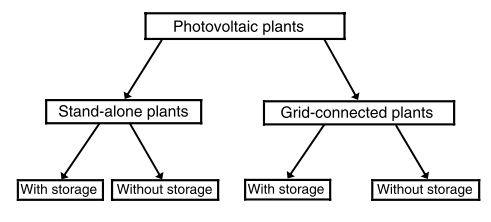
\includegraphics[width = 100mm] {images/pv-system-options}\hspace*{\fill}
	\caption{Photovoltaic Connection Options Pyramid \cite{Haberlin2012}}
	\label{fig:pv-connection-options}
\end{figure} 

%New Paragraph
Incorporating a battery into the design of the system is not extremely complicated. Figure \ref{fig:pv-connection-layouts} below shows a suggested connection option. The devices as per their numbered labels are:

\begin{enumerate}[noitemsep]
	\item Solar generator
	\item Charge controller	
	\item Battery
	\item Discharge controller
	\item DC-DC converter
	\item DC-AC converter
	\item Consumers
	\item Possible auxiliary generators (such as diesel or wind)
\end{enumerate}

\begin{figure}[H]
	\hfill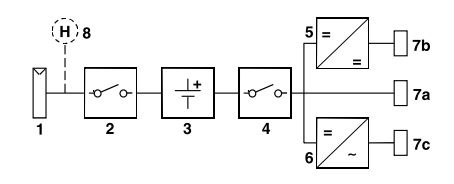
\includegraphics[width = 100mm] {images/pv-system-layout}\hspace*{\fill}
	\caption{Photovoltatic System Model with Battery Integration \cite{Haberlin2012}}
	\label{fig:pv-connection-layouts}
\end{figure} 

%New Paragraph
The storage process occurs in item 3; the battery. The nominal voltage of this device in a stand-alone system should match the installation's system voltage \cite{Haberlin2012}. There are voltage level alternatives depending on the design of the system such as 12\,V, 24\,V, 48\,V or higher for larger installations \cite{Haberlin2012}. In Australia, recent developments have seen lithium-ion battery solutions being used for solar storage far more than older technologies such as lead acid \cite{website:OffGridEnergy1}. Lithium-ion has many advantages for hybrid storage applications. They have a higher energy density and have the ability to regularly discharge \cite{website:OffGridEnergy1}. The estimated lifespan of these devices is a minimum of 15 years \cite{website:OffGridEnergy1}. A popular development in this market is the Tesla Powerwall which incorporates the same batteries that Tesla uses in their cars but in a different application \cite{Tesla1}.  

\paragraph{Converters} \label{section:litreview-converters}
~\\
%New Paragraph
Converters are electrical devices designed and constructed to convert current between AC and DC \cite{website:ConvVsInverter}. Rectifiers are used to convert the voltage from AC to DC and inverters converter from DC to AC \cite{website:ConvVsInverter}. Although these are the technical terms for the two devices, in general the term ``converter" can be used. A specific use for inverters is to convert the DC electrical generated from solar panels to AC for transfer back into mains or to the necessary switchboard. An additional use for these is in Uninterrupted Power Supplies (UPS) where DC battery power is stored and it is converted to AC when connected into existing power systems for to maintain power during grid errors \cite{website:ConvVsInverter}.

\paragraph{Buck and Boost Converters}
~\\
%New Paragraph
Buck and boost converters are a subset of the converter section above. These are used in DC to DC power systems where the voltage needs to be stepped up or stepped down \cite{textbook:Abu-Rub2014}. For smaller applications, chips such as the LM2575 buck converter are available to reduce voltages according to a feedback. Boost converters do the opposite and increase the voltage. These devices are frequently used with Photo-Voltaic systems depending on what loads they are feeding \cite{textbook:Abu-Rub2014}. The panels generate electricity that is fed through a boost converter then into an inverter to convert the electricity to AC in order to be distributed throughout the circuit \cite{textbook:Abu-Rub2014}.  

\paragraph{Direct Current Switchgear} \label{litreview:dc-devices}
~\\
%New Paragraph
Direct current devices will be required for a system that is not standard alternating current. With the increase in purely DC systems used for a variety of purposes, DC switchgear is readily available commercially. Eaton have a range of DC-DC Circuit breakers that are designed for energy storage, transportation and industrial DC circuits \cite{website:Eaton1}. Specific design mechanisms were established in order to meet the protection requirements for PV systems. 
\newline

%New Paragraph
For designs that use a large amount of DC devices, efficiency purposes suggest using a DC distribution board. There are commercially available products designed for such purposes. For example, Myers Power Products, Inc have designed a range of DC power solutions including traction power substations, DC switchgear, DC circuit breakers, rectifiers and inverters if required \cite{website:Myers1}. An example of a DC distribution room is shown in Figure \ref{fig:dc-switchgear-room}.         

\begin{figure}[H]
	\hfill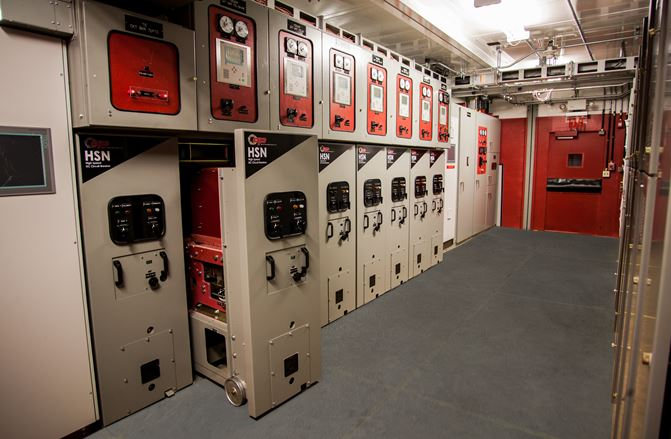
\includegraphics[width=100mm]{images/dc-switchgear}\hspace*{\fill}
	\caption{Example of DC Main Switchboard Room \cite{website:Myers1}} 
	\label{fig:dc-switchgear-room}
\end{figure}

\paragraph{LED Lighting}
~\\
%New Paragraph
Table \ref{LightingTypes} below shows a technical comparison of three common lighting types. Improvements in LED lighting allow less power to be used for the same brightness. It is possible to design and create an energy efficient Low-Voltage\,DC (LVDC) grid powered LED lighting system with additional automation aspects and energy storage \cite{Koh2011}. Typical lighting systems are fluorescent bulbs or tubes that are powered directly from standard 230 V AC due to the devices' high efficacy \cite{Koh2011}. When comparing an AC fluorescent system and a LVDC LED system, the LVDC grid system requires significantly less power conversion which increases the overall efficiency \cite{Koh2011}. The table below represents these factors. For applications, this means less physical lights are necessary for equivalent light reducing project costs \cite{website:LED}.  

\begin{table}[!ht]
	\centering
	\renewcommand{\arraystretch}{2} % Changing spacing
	\begin{tabular}{|l|c|c|c|}
		\hline
		\textbf{Lighting Type (Bulbs)} & \multicolumn{1}{l|}{\textit{Incandescent}} & \multicolumn{1}{l|}{\textit{CFL}} & \multicolumn{1}{l|}{\textit{LED}} \\ \hline
		Average Lifespan (hours) & 1,200 & 8,000 & 50,000 \\ \hline
		Wattage (at 800 lumens) & 60 & 13-15 & 6-8 \\ \hline
		Lumens/Watt & 13.3 & 53.3 & 114.3 \\ \hline
	\end{tabular} \quad
	\caption{Comparing Efficiencies of Lighting Types (Bulbs) \cite{Koh2011}}
	\label{LightingTypes}
\end{table}

\paragraph{Summary of Equipment}
~\\
Initial considerations make photovoltatic arrays a strong possibility for installation with batteries being considered if production is high enough. Additionally, batteries could be used to control load shifting if that is deemed beneficial. DC voltage regulation and level shifting will likely be required through buck and boost converters as well as rectifiers. There is DC switchgear available for purchase that specification sheets as well as drivers for LED luminaires. This further defends the hypothesis that the dedicated  extra-low voltage system will be feasible. 

%%%%%%% EQUIPMENT %%%%%%%%%%%%%
%%%%%%% EQUIPMENT %%%%%%%%%%%%%
%%%%%%% EQUIPMENT %%%%%%%%%%%%%
%%%%%%% EQUIPMENT %%%%%%%%%%%%%
%%%%%%% EQUIPMENT %%%%%%%%%%%%%
%%%%%%% EQUIPMENT %%%%%%%%%%%%%
\subsection{Photovoltatic systems}

\subsubsection{Photovoltaic Arrays and DC Arcing}
~\\
%New Paragraph
With the popularity of PV systems increasing, the risk of DC arc faults are being analysed further \cite{Spooner2008}. PV arrays and power systems are being designed with converters boosting voltages to 800\,V\,DC and 1000\,V\,DC. This is being done for efficiency and cost reduction purposes however it leads to large amounts of stress on insulation systems and arc faults developing \cite{Spooner2008}. This causes more safety concerns than traditional AC systems. There are three major causes of arc fault risk; high DC voltage, high DC current and large distribution of DC wiring \cite{website:DC-Arching}.
\newline

%New Paragraph
Photovoltaic generators are non-linear sources that vary with intensity of sunlight and behave mainly as a DC current source \cite{Ribeiro2009}. There is an additional negative of PV systems than AC due to the occurrence of DC arc faults. The DC circuits that combine to form the PV power system distribution are able to generate and sustain arcs of considerable intensities. DC arcs have their uses in applications such as welding, but for a power system they are only a risk \cite{Ribeiro2009}. The risks of DC arcs can be reduced by incorporating proper safety equipment and reducing DC voltage levels \cite{Ribeiro2009}. 

\subsubsection{Photovoltaic Mounting Solutions} \label{section:photovoltatic-mounting}

\paragraph{Fixed Mounted} 
~\\
There are multiple options for fixing modules to the selected surface areas and each has their own merit. The most popular solution are frames specifically designed to mount an array of panels on a roof, ground or other surface and keep them still in place. This is known as a fixed mounting scheme \cite{Haberlin2012}. Clips or conventional screws can be used to mount the modules to these frames. Two examples of this mounting scheme is shown in Figure \ref{fig:pv-mounting-fixed-field} and Figure \ref{fig:pv-mounting-fixed-roof}. 

\begin{figure}[H]
	\hfill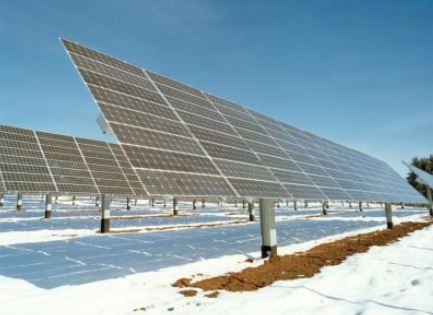
\includegraphics[width = 100mm]{images/pv-fixed-mounting}\hspace*{\fill}
	\caption{Photovoltaic System Mounting Example: Fixed  \cite{Haberlin2012}} 
	\label{fig:pv-mounting-fixed-field}
\end{figure}

\begin{figure}[H]
	\hfill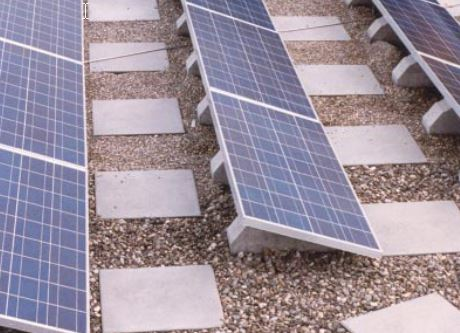
\includegraphics[width = 100mm]{images/pv-roof-mounting}\hspace*{\fill}
	\caption{Photovoltaic System Mounting Example: Roof Mounting \cite{Haberlin2012}} 
	\label{fig:pv-mounting-fixed-roof}
\end{figure}  

\paragraph{Building Integration Mounting}
~\\
There also exists creative solutions to mounting photovoltaic modules. This can be replacing roof material with modules or using them as window awnings. An example of this from the US Embassy in Geveva is shown in Figure \ref{fig:pv-mounting-fixed-windows}.  

\begin{figure}[H]
	\hfill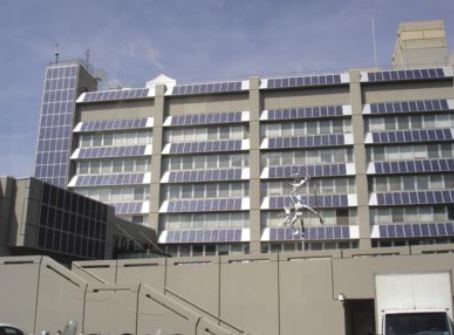
\includegraphics[width = 100mm]{images/pv-mouting-windows}\hspace*{\fill}
	\caption{Photovoltaic System Mounting Example: Window Awning \cite{Haberlin2012}} 
	\label{fig:pv-mounting-fixed-windows}
\end{figure} 

\paragraph{Single and Dual Axis Tracking System}
~\\
The yield of modules can be increased by implementing tracking systems in the modules' installations. These can be single or dual axis tracking systems. Single axis, as the name suggests, means that it will shift in one direction, back and forward, traditionally on a timer. The idea behind these is that as the day progresses, the module is able to shift to continually face the sun and receive the maximum luminance in order to increase production \cite{Haberlin2012}. An examle of this installation is shown in Figure \ref{fig:pv-mounting-single-axis}. Dual axis, again as the name suggests, shifts the module across two axes for even further increased production from the installed modules. These systems of course both require power to operate so it is possible to have a higher production than fixed axis however net production after operating the control systems could be lower.  

\begin{figure}[H]
	\hfill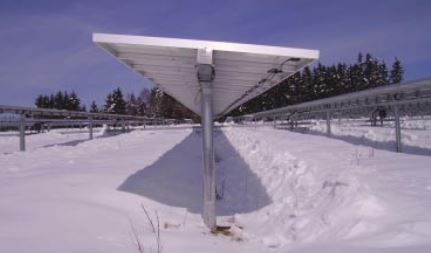
\includegraphics[width = 100mm]{images/pv-mouting-rotating}\hspace*{\fill}
	\caption{Photovoltaic System Mounting Example: Single Axis \cite{Haberlin2012}} 
	\label{fig:pv-mounting-single-axis}
\end{figure} 

\subsubsection{Summary of Photovoltaic Systems}

%New Paragraph
Photovoltaic modules will be a welcome addition to this project. Safety considerations will have to employed to prevent DC arcing in installations. For a commercial building it is likely that fixed mounting will be the ideal option due to single axis requiring larger surface areas to avoid self-shading. 

%%%%%%% EXTRA LOW VOLTAGE %%%%%%%%
%%%%%%% EXTRA LOW VOLTAGE %%%%%%%%
%%%%%%% EXTRA LOW VOLTAGE %%%%%%%%
%%%%%%% EXTRA LOW VOLTAGE %%%%%%%%
%%%%%%% EXTRA LOW VOLTAGE %%%%%%%%
%%%%%%% EXTRA LOW VOLTAGE %%%%%%%%
%%%%%%% EXTRA LOW VOLTAGE %%%%%%%%
%%%%%%% EXTRA LOW VOLTAGE %%%%%%%%


\subsubsection{Extra Low Voltage}

\paragraph{Extra-Low Voltage Direct Current}
~\\
%New Paragraph
DC power is currently restricted to special applications such as telecommunications, electric vehicles and high-voltage direct current (HVDC) transmission \cite{Salomonsson2007}. Low-voltage DC power systems at 48\,V\,DC has been used fairly widely with telecommunications systems but is recently facing issues due to the high power requirements of computer system upgrades \cite{Salomonsson2007}. Studies have shown that the 48\,V\,DC system still remains more efficient than a 270\,V\,DC or 200\,V\,AC but further investigation needs to be done into 230\,V\,DC and 325\,V\,DC through retrofitting existing low voltage AC installations \cite{Salomonsson2007}. PV generators are used frequently for these forms of power distribution systems as it can be powered directly or use simple DC to DC converters for different devices. Utilising a DC distribution system makes it easier to incorporate local power generation. This reduces costs and local power is unaffected by issues with power grid \cite{Starke2008a}. 

\paragraph{Extra-Low Voltage Direct Current in Telecommunications}
~\\
%New Paragraph
Using low voltage energy distribution grids for high-speed communications networking can open up the possibility to utilities for expansions of widespread local area networks \cite{Waldeck1998}. This could be services such as telephony and internet access without the necessity of additional cabling \cite{Waldeck1998}. Firstly, this voltage level is chosen due to it being under the maximum for low voltage power and still considered a ``safe low voltage". Additionally, this voltage level could be backed up by battery systems with four 12\,V batteries in series similar to Figure \ref{fig:48VTelecomms}. Many data centres or communications rooms for corporate buildings will establish arrays of 48\,V battery banks \cite{website:48VTelecomms}. A solution for areas without large enough storage areas for are limited and power demands are low a single 12\,V battery with a 12\,V to 48\,V boost converter can be used \cite{website:48VTelecomms}. This setup is shown in Figure \ref{fig:48VTelecomms}. Additionally, due to this nature of power telecomms, standalone systems are becoming a more suitable means of supply \cite{Ribeiro2009}. Photovoltaic arrays, due to their DC source nature, could be used with a DC to DC boost converter and regulator to power these systems.   

\begin{figure}[H]
	\hfill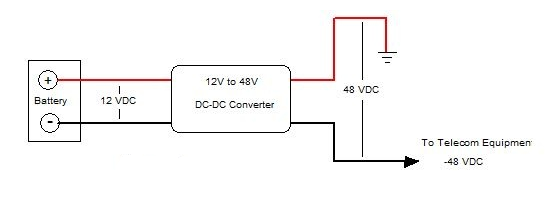
\includegraphics[width = 100mm]{images/12V_Telecomms.png}\hspace*{\fill}
	\caption{12\,V\,DC Battery Backup with 12 to 48\,V\,DC Converter in Telecommunications \cite{website:48VTelecomms}}
	\label{fig:48VTelecomms}
\end{figure}  

\paragraph{Electrical Safety in Low Voltage DC}
~\\
%New Paragraph
Fuses, mechanical and electronic safety switches / circuit breakers and their combinations operate the same in DC as they do in AC; detecting electric faults and switching off to isolate electrical equipment \cite{Meckler2014}. Plugs, sockets and safety equipment with nominal currents of 20 \si{A} are commercially available for pre-existing DC data centres \cite{Meckler2014}. 

\paragraph{Summary of Extra Low Voltage}
~\\
Specific considerations are required for the use of extra-low DC voltage. Extra Low Voltage is deemed as voltage levels under 50\,V. 48\,V\,DC is a commonly used voltage level and has several successful case studies available. Due to the extensive research into these systems, commericially available products as well support the voltage level and data can be found on how to accurately model these systems. 

%%%%%%% END %%%%%%%%%%%%%

\newpage